\documentclass[11pt,a4paper]{article}
\author{TalentSprint}
\date{}
\usepackage{verbatim}
\usepackage{fancyhdr}           % For header and footer
\usepackage{multicol}
\usepackage{colortbl}           % For coloured tables
\usepackage{setspace}           % For line height
\usepackage{seqsplit}           % Splits long words.
\usepackage{amsmath} 
\usepackage{graphicx}
\usepackage{array}
\usepackage{enumitem}
\usepackage{xcolor}
\usepackage[tikz]{bclogo}
\usepackage{textcomp}
\usepackage{listings}
\lstset{language=python,numbers=left,numberstyle=\tiny,numbersep=10pt,showstringspaces=false}

\headheight=14pt
\lhead{\nouppercase{}}
\rhead{\nouppercase{\leftmark}}

\newcommand*\lstinputpath[1]{\lstset{inputpath=#1}}
\lstinputpath{../Code/}
\graphicspath{{../Images/} {../ScreenShots/}}

\setcounter{tocdepth}{1}
\setlength\parindent{0pt}
\parskip=4pt
\newcommand{\Code}[1]{\textbf{\texttt{#1}}}

% Lengths and widths
\addtolength{\textwidth}{5cm}
\addtolength{\hoffset}{-1cm}
\setlength{\headsep}{-12pt} % Reduce space between header and content
\setlength{\headheight}{85pt} % If less, LaTeX automatically increases it
\renewcommand{\footrulewidth}{2pt} % Remove footer line
\renewcommand{\headrulewidth}{1pt} % Remove header line
\renewcommand{\seqinsert}{\ifmmode\allowbreak\else\-\fi} % Hyphens in seqsplit
% This two commands together give roughly
% the right line height in the tables
\renewcommand{\arraystretch}{1.3}
\onehalfspacing

% Commands
\newcommand{\SetRowColor}[1]{\noalign{\gdef\RowColorName{#1}}\rowcolor{\RowColorName}} % Shortcut for row colour
\newcommand{\mymulticolumn}[3]{\multicolumn{#1}{>{\columncolor{white}}#2}{#3}} % For coloured multi-cols
\newcolumntype{x}[1]{>{\raggedright}p{#1}} % New column types for ragged-right paragraph columns
\newcommand{\tn}{\tabularnewline} % Required as custom column type in use

% Font and Colours
\definecolor{HeadBackground}{HTML}{333333}
\definecolor{FootBackground}{HTML}{666666}
\definecolor{TextColor}{HTML}{333333}
\definecolor{DarkBackground}{HTML}{6B8E23} %{FD1AA8}
\definecolor{LightBackground}{HTML}{E8FED8} %D3FDC8
\definecolor{tit}{HTML}{FF6600}
\renewcommand{\familydefault}{\sfdefault}
\color{TextColor}
 \headsep = 25pt
% Header and Footer
\pagestyle{fancy}
\usepackage[headheight=110pt]{geometry}
\fancyhf{}% Clear header/footer

\fancyhead[r]{
\includegraphics[width = 4cm, height = 2cm]{TS-Logo.png}\hspace{0cm}}

%=================================TITLE=====================================
\fancyhead[l]{\Large{\bf{\textcolor{tit}{\textrm{Function Decomposition}}}}}
%===========================================================================

\renewcommand{\headrulewidth}{0.4pt}% Default \headrulewidth is 0.4pt
\renewcommand{\footrulewidth}{0.4pt}% Default \footrulewidth is 0pt

\rfoot{Page \thepage}
\lfoot{COPYRIGHT \textcopyright TALENTSPRINT, 2015. ALL RIGHTS RESERVED.}




\begin{document}


%\chapter{Functional Decomposition}
Typical commercial systems are very large. When the size of a codebase increases the difficulties in avoiding errors, making changes and so on also increase significantly.  By segmenting the program into  clearly defined functions, we can address these problems, as well as improve reusability of code.

What do we mean by a well-defined function? ``Do one task and not do similar but unrelated tasks'' is one good maxim. We will note other guidelines as we go along.

\section*{Functions}
A function is a piece of code that performs a particular task. Instead of writing this block of code inside a larger chunk of code, we give it a \emph{good} name and put it into a function. 

In other words, functions help us to split up a long program into named sections so that the section can be reused --in the same program as well as in other programs.

\subsection*{main()}
Every C program consists of one special function called \texttt{main()}. Execution will always start from \texttt{main()}.

\subsection*{Categories Of Functions}
C functions can be classified into two categories,
\begin{description}
\item [Built-in Functions]
These functions are also called as `library functions'. Library functions are those functions which are defined by C library, or external (`third party') libraries, example \texttt{printf(), scanf(), strcat()} etc. You just need to include appropriate header files to use these functions. These are already declared and defined in C libraries.

For example, all standard I/O functions are available in \emph{\textless stdio.h \textgreater}. Mathematical functions are in \emph{\textless math.h \textgreater}. 
String handling functions are in \emph{\textless string.h \textgreater}.

Once again:
\begin{itemize}
  \item whenever you want to use any library function in your program include the corresponding header file before \texttt{main()} and
  \item indicate the library required. For example, \textbf{\texttt{c99 -lm compute.c}}, compiles and links a program \texttt{compute.c} that uses  math library functions.  
\end{itemize}

\item [User-defined Functions]
User-defined functions are those functions which are defined by the user at the time of writing the program. Such functions are made for code reusability and for saving time and space.
\end{description}

\subsection*{Declaration} 

Every function we use must be declared before it is used -- as we have noted, the header files handle the declaration for built-in functions. The actual body of the function can be defined separately. 

For functions we write, we can either add a declaration line at the top of the program or put the declaration in a header file of our own and include that header file. The second method is appropriate when we are writing a suite of related functions, the first is sufficient for most of our purposes in the early stages. 

General syntax of function declaration is: 

\textbf{\texttt{return\_type function\_name(parameter-list);}}

A function declaration is similar to a variable declaration. It tells the compiler about the function: its name, and how to call it. It also helps the compiler to detect wrongly written invocations. 

A function declaration consists of 4 parts.
\begin{enumerate}
\item return-type
\item function name
\item parameter list
\item terminating semicolon
\end{enumerate}

\subsection*{Definition} 

General syntax of function definition is:

\begin{lstlisting}[numbers=none]
    return_type function_name (parameter-list) {   
        function-body;
    }
\end{lstlisting}

The first line  known as function header and the statement(s) within braces are called \emph{function body}.

\begin{description}
\item [return-type] return type specifies the type of value (\emph{int, float, char, double}) that the function is expected to return to the program calling the function.
Some functions perform the desired operations without returning a value. In this case, the return type is the keyword \lstinline!void!\footnote{Technically such functions are known as \emph{procedures}}.

\item [function-name]
function name specifies the name of the function. The function name is any valid C identifier and therefore must follow the same rules of naming as other variables in C. The function name and the parameter list together constitute the \emph{function signature}. 

\item [parameter-list]
The parameter list refers to the type, order, and number of the parameters of a function. The parameter list declares the variables that will receive the data sent by calling program. They are often referred to as \emph{formal parameters}. These are separated by commas.

\item [function-body]
The function body contains the declarations and the statements necessary for performing the required task. The body is enclosed within curly braces \{ \} and consists of three parts.

\begin{itemize}
\item local variable declaration,
\item statements that perform the tasks of the function, and
\item a \lstinline!return! statement that returns the value evaluated by the function. (Or a empty \lstinline!return! for a procedure).
\end{itemize}
\end{description}

\subsection*{Calling} 
Control of the program is transferred to user-defined function by \emph{calling} it (invoking). Arguments are the values specified during the function call, for which the formal parameters are declared in the function. The number of arguments must match the number of formal parameters and must be of the same (or equivalent) data type.

\begin{figure}[ht]

\begin{center}
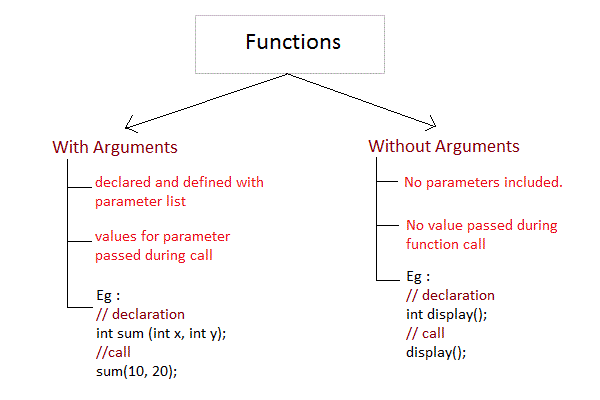
\includegraphics[scale = 0.5]{functions-and-arguments.png}
\caption{Invocation: With and Without Arguments}
\label{Invocation}
\end{center}
\end{figure}

\subsubsection*{Example} 
\lstinputlisting{Program-08-1.c}

\begin{figure}[ht]
\label{output-08-1}
\begin{center}
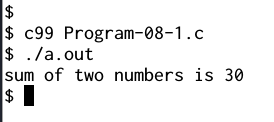
\includegraphics[scale=0.6]{Output-08-1.png}
\caption{Using Function}
\end{center}
\end{figure}

\begin{bclogo}[couleur=blue!5, arrondi=0.3, logo=\bctrombone]{Benefits of using functions}
\begin{itemize}
\item User defined functions help to decompose the large program into small segments. This makes programs easy to understand, maintain and debug.
\item Easy code Reuseability. You just have to call the function by its name to use it.
\item It provides modularity to the program.
\item It reduces the size of a program and easy to understand the actual logic of a program.
\end{itemize}
\end{bclogo}

\section*{Code Reading}
\subsection*{Primes in Range}
A program to Display Prime Numbers in a given range.

The following three step approach should be used a general guideline to think and plan tour programs.

\begin{enumerate}
  \item Identify functions needed; 
    \begin{itemize}
    \item describe their purpose 
    \item determine what information they need for that
    \item choose a name
    \end{itemize}
  \item Implement the functions 
  \item Put the functions together to do the whole task
\end{enumerate}

In this case, we can see that we need a function to check if a given number is prime, we can simply run a loop over the range and call that function.

We are looking for an output like this:
\begin{figure}[ht]
\begin{center}
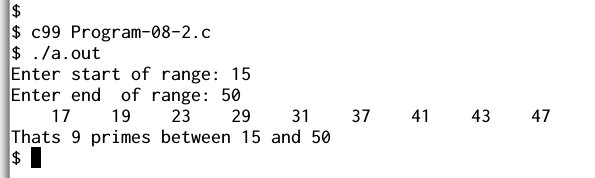
\includegraphics[scale=0.6]{Output-08-2.png}
\caption{Primes In Range}
\label{output-08-2}
\end{center}
\end{figure}

Now let us actually write the code, adding a main which accepts the range and calls the function.

\lstinputlisting{Program-08-2.c}


\end{document}